\subsection{Probabilistic Mediated Schema Mapping}
\textcolor{red}{\textbf{TODO}}\\
\textcolor{red}{Used Papers: \cite{DasSarma:2008:BPD:1376616.1376702}}

In \cite{DasSarma:2008:BPD:1376616.1376702} was shown, that it is possible to automatically bootstrap a data integration system that answers queries with high precision and recall. In a sense, it is possible to set up a data integration system without any human involvement. With this approach, it isn't possible to answer queries fully accurate and complete as it would be with manual or semi-automatic ones, but best-effort answers and improvement over time are possible by using a probabilistic data model. 
Mediated schemas can be build automatically by clustering attributes from the various source schemas to groups by their semantic meaning and then using this groups as attributes in the mediated schema. Sources in a dataspace typically are heterogeneous, so as a general rule there is more than one possibility to cluster the attributes and it exists an uncertainty of the best(s) grouping(s). If you would choose only one schema of the set of possible mediated schemas, you would likely have a loss in query answering in both terms, precision and recall.  So it seems natural to consider all possible mediated schemas combined in a single mediated schema. By weighting each mediated schema through its likelihood of accuracy, it is possible to favor schemas with a greater weight for query answering and answer ranking. And that is exactly, what a probabilistic mediated schema (p-mediated schema) is doing.
For clustering attributes from the source schemas, similarity functions based on attribute matching are used. Thus, some not very obvious attribute correspondences aren't detected by this approach. But the authors believe, that using more advanced schema matching algorithms like also considering column value similarities, could minimize this problem \cite{DasSarma:2008:BPD:1376616.1376702}.

The concept of probabilistic Schema Mapping (p-mapping) was introduced in \textcolor{red}{Cite!!!}. It describes a probabilistic distribution of possible mappings between a source and a mediated schema. A mathematical formal definition and additional information about probabilistic schema mapping can be found in the original paper \cite{DasSarma:2008:BPD:1376616.1376702}.
 
The whole process is visually represented in \ref{BootstrappingPayAsYouGoDISystems1}, which shows the architecture of the data integration system used by \cite{DasSarma:2008:BPD:1376616.1376702}.

\begin{figure}[H]
	\begin{center}
		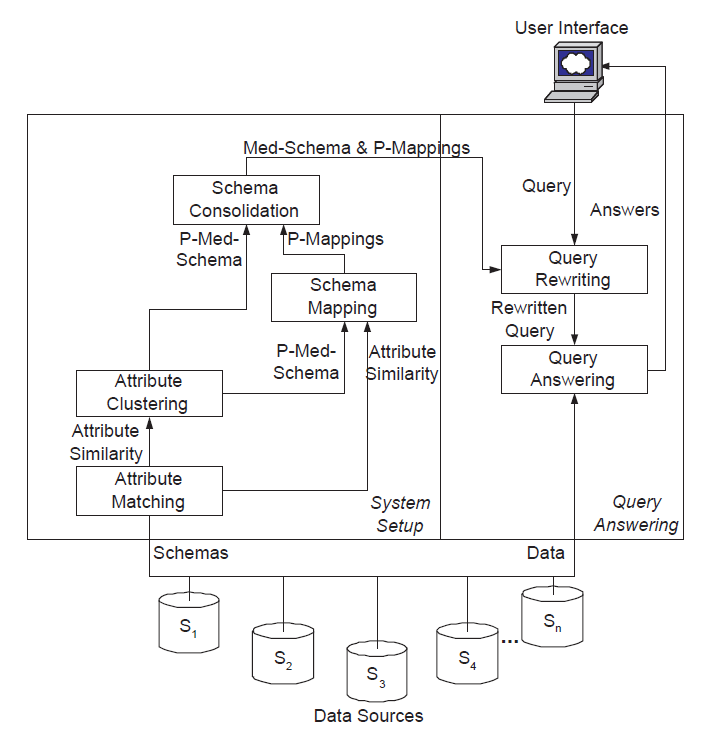
\includegraphics[width=0.75\textwidth]{figures/BootstrappingPayAsYouGoDISystems1.png}
	\end{center}
	\caption{Bootstaping a 'Pay as you go' data integration system}
	\label{BootstrappingPayAsYouGoDISystems1}
\end{figure}

On set-up time, the system automatically generates the p-mediated schema and appertaining p-mappings by clustering the attributes of the source schemas and calculating mapping probabilities afterwards. For the clustering process similarity functions are used, but more advanced techniques could used, as well. After creating the p-mediated schema and its p-mappings, they are consolidated to generate a final mediated schema and p-mappings. Consolidation means to aggregate all possible schemas to one mediated schema and creating p-mappings for this single schema. The purpose of the consolidation is providing the user a sole mediated schema to interact with and additionally it speeds up query answering, as the consolidation process removes redundant information from the p-mediated schema and therefore queries only need to be rewritten and answered based on one mediated schema.
At query-answering time the query is rewritten for each data source according to the mappings and answers the rewritten query on the data sources. Answering queries with respect to p-mappings returns a set of answer tuples, each with a probability indicating the likelihood that the tuple occurs as an answer.

As probabilistic schema mapping is crucial for dataspace systems we want to go a little more in depth by showing a little example of bootstrapping a fictional data integration system providing access to bio-medical information in the field of antimicrobial susceptibility tests:

Let us assume we have 2 data sources S\textsubscript{1} and S\textsubscript{2} . 
Their concepts and data sets are shown in \ref{PMappingExampleConcepts}.

\begin{figure}[H]
	\begin{center}
		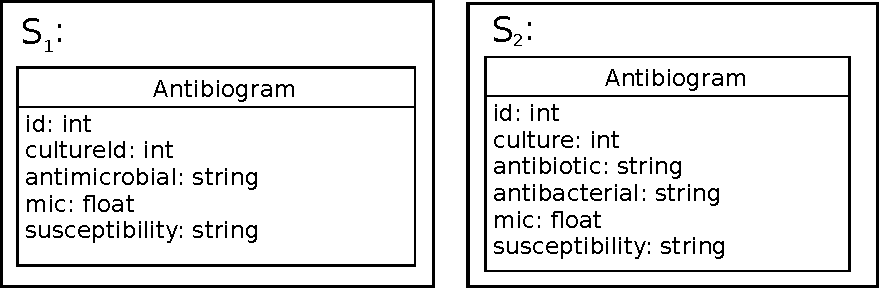
\includegraphics[scale=0.75]{figures/PMappingExampleConcepts.pdf}
	\end{center}
	\caption{Concepts of our example}
	\label{PMappingExampleConcepts}
\end{figure}

Beside syntactic heterogeneity,  the attribute members \textit{antibiotic} and \textit{antibacterial} from S\textsubscript{2} could both possibly matched to \textit{antimicrobial} from S\textsubscript{1}. Clustering using similarity function could thereby result in the following two clusterings (other possibilities are omitted for the sake of simplicity):

M\textsubscript{1}: (\{\textit{id}\}, \{\textit{cultureId}, culture\}, \textit{drug} := \{\textit{antimicrobial}, antibiotic\}, \{antibacterial\}, \{mic\}, \{susceptibility\})\\
M\textsubscript{2}: (\{\textit{id}\}, \{\textit{cultureId}, culture\},  \textit{drug} := \{\textit{antimicrobial}, antibacterial\}, \{antibiotic\}, \{mic\}, \{susceptibility\})

To break it down, the two clusterings show whether \textit{antibiotic} or \textit{antibacterial} are semantically equal to \textit{antimicrobial}. Let us assume that both schemas are equally probable, this means $ P(M\textsubscript{1}) = P(M\textsubscript{2}) =  \frac{1}{2} $.\\
Consequently the p-mediated schema is given by:\\
$M\textsubscript{P}: \{(M\textsubscript{1}, \frac{1}{2}), (M\textsubscript{2}, \frac{1}{2})\}$\\
\raggedright
The appertaining p-mappings are given by \ref{Probabilities-p-mapping} (note, that the probabilities are only for demonstration purposes and weren't calculated):\\
%\begin{table}[]
\centering
\begin{tabular}{|p{0.8\textwidth}|p{0.2\textwidth}|}
\hline
 \textbf{Possible Mapping for M\textsubscript{1}}  &  \textbf{Probability}\\ \hline
 m\textsubscript{11} := \{(id, id), (culture, cultureId), (antibiotic,  \textit{drug}), (antibacterial, antibacterial), (mic, mic), (susceptibility, susceptibility)\}   &  $ \frac{9}{10} $\\ \hline
 m\textsubscript{12} :=  \{(id, id), (culture, cultureId), (antibacterial,  \textit{drug}), (antibiotic, antibacterial), (mic, mic), (susceptibility, susceptibility)\}   &  $ \frac{1}{10} $\\ \hline
\end{tabular}
\begin{tabular}{|p{0.8\textwidth}|p{0.2\textwidth}|}
\hline
 \textbf{Possible Mapping for M\textsubscript{2}}  &  \textbf{Probability}\\ \hline
  m\textsubscript{21} := \{(id, id), (culture, cultureId), (antibacterial,  \textit{drug}), (antibiotic, antibiotic), (mic, mic), (susceptibility, susceptibility)\}   &  $ \frac{8}{10} $\\ \hline
  m\textsubscript{22} := \{(id, id), (culture, cultureId), (antibiotic,  \textit{drug}), (antibacterial, antibiotic), (mic, mic), (susceptibility, susceptibility)\}   &  $ \frac{2}{10} $\\ \hline
\end{tabular}
\captionof{table}{Probabilities of the p-mappings}
\label{Probabilities-p-mapping}
%\end{table}
\raggedright
Now, let's assume, we have the following data set in S\textsubscript{2} containing only one tuple: \{(3180102, 1910181, cefepime, axepim, 0.96, S)\};
And assume we want to process the query:\newline\\

\textbf{Select} drug, mic, susceptibility\\
\textbf{from } Antibiogram\newline\\

Using the schemas M\textsubscript{1} and M\textsubscript{2}, the possible answers would be:
\textit{a\textsubscript{1}} := (cefepime, 0.96, S)\\
\textit{a\textsubscript{2}} :=  (axepim, 0.96, S)\\
\raggedright
To calculate their probabilities and therefore getting the order for a Top-k ranking, we have to consider both, the probability of the schemas and their attending p-mappings. Therefore:\\
$P(a\textsubscript{1}) = P(M\textsubscript{1}) \cdot P(m\textsubscript{11}) + P(M\textsubscript{2}) \cdot P(m\textsubscript{22}) = \frac{1}{2} \cdot \frac{9}{10} + \frac{1}{2} \cdot \frac{2}{10} = \frac{11}{20}$\newline
$P(a\textsubscript{2}) = P(M\textsubscript{1}) \cdot P(m\textsubscript{12}) + P(M\textsubscript{2}) \cdot P(m\textsubscript{21}) = \frac{1}{2} \cdot \frac{1}{10} + \frac{1}{2} \cdot \frac{8}{10} = \frac{9}{20}$\newline
\\
Finally, the top-k answer looks like:\\
{
\centering
\begin{tabular}{|p{0.4\textwidth}|p{0.2\textwidth}|}
\hline
 \textbf{Answer}  &  \textbf{Rank}\\ \hline
  (cefepime, 0.96, S)  &  0.55 \\ \hline
  (axepim, 0.96, S)  &   0.45\\ \hline
 \hline
\end{tabular}
\captionof{table}{Query answer of our example}
\label{query-answer-top-k}
}